%usepackage es egyebek
\pdfminorversion=4
\documentclass[17pt]{extarticle}

\usepackage[margin=1.5cm,nohead]{geometry}
\usepackage[utf8]{inputenc}
%	\usepackage[hungarian]{babel}


\usepackage[%hypertex,
   unicode=true,
   plainpages = false,
   pdfpagelabels,
   bookmarks=true,
   bookmarksnumbered=true,
   bookmarksopen=true,
   breaklinks=true,
   backref=false,
   colorlinks=true,
   linkcolor = blue,
   urlcolor  = blue,
   citecolor = red,
   anchorcolor = green,
   hyperindex = true,
   hyperfigures,
%   pdftex
]{hyperref}
\hypersetup{
   pdftitle={Feladatok},
   pdfauthor={Czylabson Asa},
   pdfsubject={Hold Föld Nap},
}


\usepackage{amsmath}
\usepackage{amsfonts}
\usepackage{amssymb}
\usepackage{graphicx}
\usepackage{type1cm}
\usepackage{setspace}
\usepackage{mathtools}


%\usepackage{xcolor}
%\usepackage{tikz,lipsum,lmodern}
\usepackage[most]{tcolorbox}


\usepackage{matlab-prettifier}
\usepackage[T1]{fontenc}
\usepackage{listingsutf8}

\lstset{
   style              = Matlab-editor,
   basicstyle         = \mlttfamily,
   escapechar         = ",
   mlshowsectionrules = true,
   literate= {á}{{\'{a}}}1 {Á}{{\'{A}}}1 {é}{{\'{e}}}1 {É}{{\'{E}}}1 {í}{{\'{i}}}1 {Í}{{\'{I}}}1 {ó}{{\'{o}}}1 {Ó}{{\'{O}}}1  {ö}{{\"{o}}}1 {Ö}{{\"{O}}}1 {ő}{{\H{o}}}1 {Ő}{{\H{O}}}1 {ú}{{\'{u}}}1 {Ú}{{\'{U}}}1  {ü}{{\"{u}}}1 {Ü}{{\"{U}}}1 {ű}{{\H{u}}}1 {Ű}{{\H{U}}}1
}

%https://tex.stackexchange.com/questions/254324/how-to-creat-color-boxes-as-the-picture
% FASZ = feladatszín
\definecolor{FASZ}{RGB}{160, 187, 229}
%\definecolor{LESZ}{RGB}{206, 177, 224} ez lilás
% leiras (desc) szine
\definecolor{LESZ}{RGB}{173, 173, 235}
% megoldas
\definecolor{MOSZ}{RGB}{102, 209, 141}
% link szine
\definecolor{LISZ}{RGB}{232, 219, 106}
%\definecolor{MASZ}{RGB}{217, 210, 221}
% matek mod szine
\definecolor{MASZ}{RGB}{210, 203, 214}
%\definecolor{BGSZ}{RGB}{224,224,224} szurke
\definecolor{BGSZ}{RGB}{220,220,220} 
\definecolor{VKEK}{RGB}{225,235,255} 
\definecolor{VBAR}{RGB}{255,240,230} 


\newcommand{\feher}[1]{%
\begin{tcolorbox}[colback=white]
#1
\end{tcolorbox}
}

\newcommand{\matlab}[1]{%
\feher{\lstinputlisting{DB/M/#1.m}}
}

\newcommand{\egykep}[1]{%
\begin{center}
\makebox[\textwidth]{\includegraphics[width=\textwidth]{DB/fig/#1}}
\end{center}
}

\newcommand{\szinesdoboz}[2]{%
\begin{tcolorbox}[colback=#1]
#2
\end{tcolorbox}
}



\newcommand{\zold}[1]{%
\begin{tcolorbox}[colback=green!17]
#1
\end{tcolorbox}
}

\newcommand{\szurke}[1]{%
\begin{tcolorbox}[colback=gray!10!white]
#1
\end{tcolorbox}
}

\newcommand{\szurkeM}[1]{%
\begin{tcolorbox}[colback=gray!10!white, top=-5mm, bottom=3mm]
\begin{gather*}
#1
\end{gather*}
\end{tcolorbox}
}

\newcommand{\Mat}[1]{%
\begin{tcolorbox}[colback=MASZ, top=-5mm, bottom=2mm, enlarge bottom finally by=-3mm]
\begin{gather*}
#1
\end{gather*}
\end{tcolorbox}
}

\newcommand{\MatTag}[2]{%
\begin{tcolorbox}[colback=MASZ, top=-5mm, bottom=3mm]
\begin{gather*}\label{#1}\tag{#1}
#2
\end{gather*}
\end{tcolorbox}
}


\newcommand{\LINK}[1]{%
\begin{tcolorbox}[colback=LISZ]
#1
\end{tcolorbox}
}

\newcommand{\barna}[1]{%
\begin{tcolorbox}[colback=brown!20!white]
#1
\end{tcolorbox}
}

\newcommand{\kek}[1]{%
\begin{tcolorbox}[colback=blue!20!white]
#1
\end{tcolorbox}
}

\newcommand{\Fa}[1]{%
\begin{tcolorbox}[colback=FASZ]
#1
\end{tcolorbox}
}

\newcommand{\Fnew}[0]{%
\end{tcolorbox}
\begin{tcolorbox}[colback=FASZ]
}

\newcommand{\Desc}[1]{%
\begin{tcolorbox}[colback=LESZ]
#1
\end{tcolorbox}
}

\newcommand{\Dnew}[0]{%
\end{tcolorbox}
\newpage
\begin{tcolorbox}[colback=LESZ]
}


\newcommand{\Mo}[1]{%
\begin{tcolorbox}[colback=MOSZ]
#1
\end{tcolorbox}
}


\newcommand{\Mnew}[0]{%
\end{tcolorbox}
\begin{tcolorbox}[colback=LESZ]
}


\newcommand{\egyFa}[1]{%
\Fa{\input{#1Fa}}
\Mo{\input{#1Mo}}
}

\newcommand{\egyDesc}[1]{%
\Desc{\input{#1Desc}}
}




\definecolor{light-gray}{gray}{0.95}
\newcommand{\mcode}[1]{
   \colorbox{light-gray}{\texttt{#1}}
}

\newcommand{\mmcode}[1]{
   {\colorbox{VBAR}{#1}}
}

\newlength{\mlen}
\settowidth{\mlen}{12345}
\newcommand{\mtit}[1]{
   \makebox[\mlen][r]{\color{gray}#1 }
}

% ez valahol kellett
\DeclarePairedDelimiter\ceil{\lceil}{\rceil}
\DeclarePairedDelimiter\floor{\lfloor}{\rfloor}

% zárójelek stb.
\newcommand{\Gzjel}[1]{%
{ \left( #1 \right) }
}

\newcommand{\gzjel}[1]{%
{ \left( #1 \right) }
}

\newcommand{\Toligv}[2]{%
#1,\hdots ,#2
}

\newcommand{\GZJ}[1]{%
{ \left( #1 \right) }
}

\newcommand{\KZJ}[1]{%
{ \{ #1 \} }
}

\newcommand{\szzjel}[1]{%
{ \left[ #1 \right] }
}

\newcommand{\Tolig}[2]{%
#1\hdots #2
}

\newcommand{\SZOR}[2]{%
#1\cdot\hdots\cdot #2
}

% integrál rendes d-vel
\newcommand{\mint}[2]{%
\int #1 \text{d}#2
}

\newcommand{\mder}[2]{%
\frac{\text{d} #1}{\text{d}#2}
}


% ez máshogy van alapban
\newcommand{\tg}[0]{%
\tan
}

\newcommand{\ctg}[0]{%
\cot
}

\newcommand{\D}[1]{%
{{\mathbb{D}\szzjel{#1}}}
}

\newcommand{\V}[1]{%
{{{\mathbb{D}}^{2}\szzjel{#1}}}
}


\newcommand{\E}[1]{%
{{\mathbb{E}\szzjel{#1}}}
}

\newcommand{\A}[1]{%
{\mathbb{A}\szzjel{#1}}
}

\newcommand{\hehu}[1]{%
\hspace{0.5cm}#1\hspace{0.5cm}
}

\newcommand{\bmx}[1]{%
\begin{bmatrix}
#1
\end{bmatrix}
}

\newcommand{\mx}[1]{%
\begin{matrix}
#1
\end{matrix}
}

\newcommand{\gjmx}[2]{%
\left[
\begin{array}{@{}c|c@{}}
#1 & #2
\end{array}
\right]
}




% rövid alakok a hosszabb szavakra
\newcommand{\fv}[1]{%
függvény#1
}

\newcommand{\Fv}[1]{%
Függvény#1
}

\newcommand{\der}[1]{%
derivált#1
}

\newcommand{\Der}[1]{%
Derivált#1
}

\newcommand{\de}[1]{%
differenciálegyenlet#1
}

\newcommand{\De}[1]{%
Differenciálegyenlet#1
}

\newcommand{\kef}[1]{%
kezdeti érték feladat#1
}

\newcommand{\Kef}[1]{%
Kezdeti érték feladat#1
}


\newcommand{\amgm}[1]{%
számtani-mértani közép#1
}
\newcommand{\Amgm}[1]{%
Számtani-mértani közép#1
}
\newcommand{\gmhm}[1]{%
mértani-harmonikus közép#1
}
\newcommand{\Gmhm}[1]{%
Mértani-harmonikus közép#1
}

\newcommand{\amqm}[1]{%
számtani-négyzetes közép#1
}
\newcommand{\Amqm}[1]{%
Számtani-négyzetes közép#1
}


\newcommand{\szigmon}[1]{%
szigorúan monoton#1
}
\newcommand{\Szigmon}[1]{%
Szigorúan monoton#1
}
\newcommand{\nov}[1]{%
növekvő#1
}
\newcommand{\Nov}[1]{%
Növekvő#1
}

\newcommand{\elen}[1]{%
egyenlőtlenség#1
}

\newcommand{\Elen}[1]{%
Egyenlőtlenség#1
}

\newcommand{\vv}[1]{%
valségi változó#1
}

\newcommand{\Vv}[1]{%
Valségi változó#1
}

\newcommand{\leb}[0]{%
lebegőpontos
}

\newcommand{\Leb}[0]{%
Lebegőpontos
}

\newcommand{\Omkd}[1]{%
Oldja meg a következő differenciálegyenletet#1
}



% helyek horizontalis
\newcommand{\kkh}[0]{%
\hspace{0.2cm}
}

\newcommand{\kh}[0]{%
\hspace{0.4cm}
}

\newcommand{\nh}[0]{%
\hspace{0.8cm}
}

\newcommand{\nnh}[0]{%
\hspace{1.0cm}
}


%ujsor
\newcommand{\us}[0]{%
\\[1ex]
}
\newcommand{\nus}[0]{%
\\[2ex]
}
\newcommand{\kus}[0]{%
\\[-1ex]
}




\hyphenation{-transz-for-mált-ját}

\newcommand{\opover}[2]{%
\kh \overset{ #1 }{ #2 } \kh
}
\newcounter{felszam}

\newcommand{\feladat}[0]{%
\stepcounter{felszam}
\noindent {\bf \arabic{felszam}. Feladat }
}

\newcommand{\magy}[0]{%
\noindent {\bf Magyarázat }
}

\newcommand{\sect}[1]{%
\noindent {\newline \bf #1 \newline}
}


\begin{document}
\sect{Emlékeztető}
\begin{spacing}{1.3}
\begin{gather*}
F(\omega) = \mhint{-\infty}{\infty}{f(t)e^{-i\omega t}}{t}\\
e^{it}=\cos(t)+i\sin(t)\\
\mhint{a}{b}{A(t)+iB(t)}{t}=
\mhint{a}{b}{A(t)}{t}+i\mhint{a}{b}{B(t)}{t}
\end{gather*}
\end{spacing}
\sect{Jelölés}
$FT$ = Fourier-transzformált\\


\sect{Feladatok}
\feladat Számoljuk ki a következő \fv{}$FT$-ját:
\begin{equation*}
f(t) =
   \begin{cases*}
      1 & $-\frac{1}{2} \le t \le \frac{1}{2}$\\
      0        & egyébként
   \end{cases*}
\end{equation*}
\sect{Megoldás}
\begin{gather*}
\mhint{-\infty}{\infty}{f(t) e^{-i\omega t}}{t} \opover{1.}{=}
\mhint{-0.5}{0.5}{e^{-i\omega t}}{t} \opover{2.}{=}
\mhint{-0.5}{0.5}{\cos(-\omega t)}{t} \opover{3.}{=}\us
\opover{3.}{=} 2\mhint{0}{0.5}{\cos(\omega t)}{t} \opover{4.}{=}
2\mhpfv{0}{0.5}{\frac{\sin(\omega t)}{\omega}}
\opover{4.}{=} \frac{\sin(\frac{\omega}{2})}{\frac{\omega}{2}}
\us
\end{gather*}
\magy
\begin{enumerate}
\item definíciók
\item $f(t)\sin(t)$ \kh páratlan
\item $\cos(\omega t)$ és $\vert t\vert \cos(\omega t)$ \kh páros
\item integrálás, behelyettesítés
\end{enumerate}

\feladat Ábrázoljuk az előző feladat \fv{ét}és $FT$-ját!
\sect{\href{negyszog.m}{Megoldás}}
%~ \lstinputlisting[style=Matlab-editor]{negyszog.m}
\begin{center}
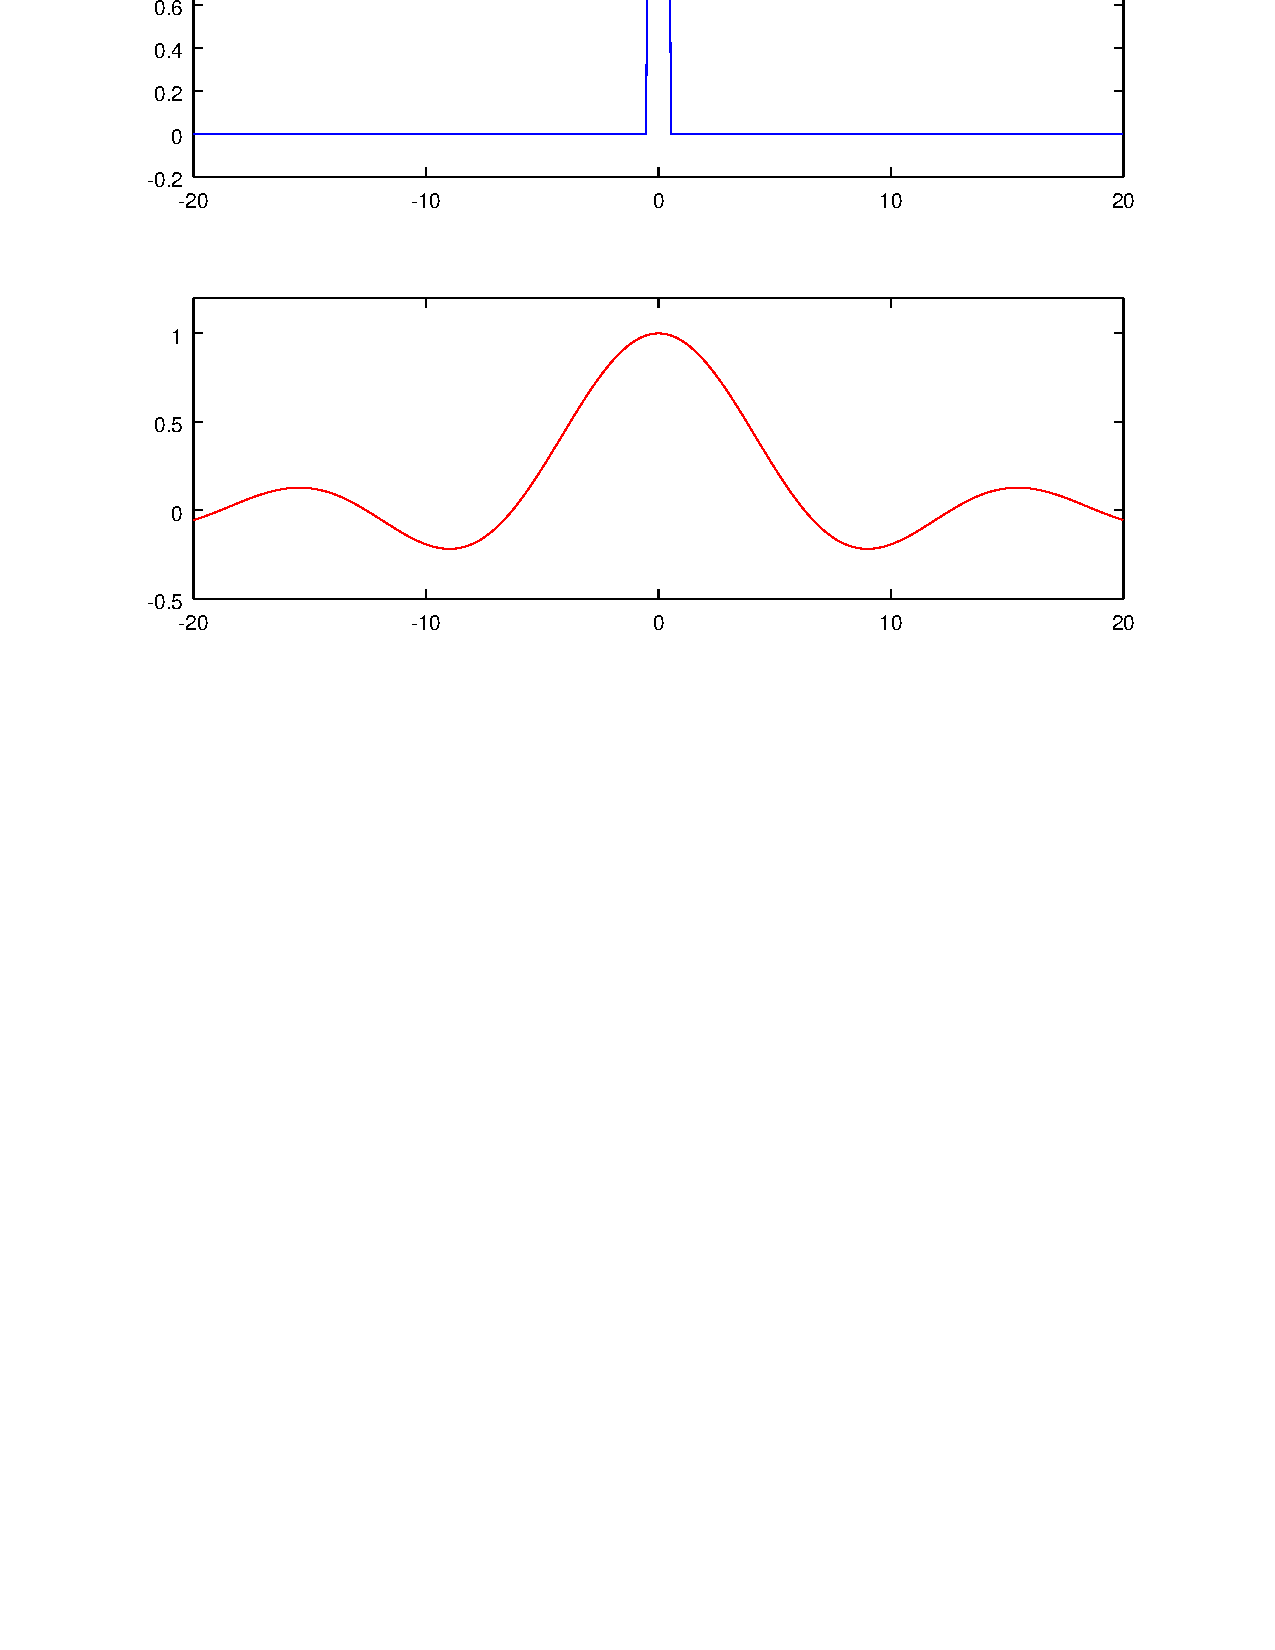
\includegraphics[scale=0.9]{negyszog}
\end{center}


\feladat Számoljuk ki a következő \fv{}$FT$-ját!
\begin{equation*}
f(t) =
   \begin{cases*}
      \vert t \vert & $-1 \le t \le 1$\\
      0        & egyébként
   \end{cases*}
\end{equation*}
\sect{Megoldás}
\begin{gather*}
\mhint{-\infty}{\infty}{f(t) e^{-i\omega t}}{t} \opover{1.}{=}
\mhint{-1}{1}{\vert t \vert e^{-i\omega t}}{t} \opover{2.}{=}
\mhint{-1}{1}{\vert t\vert \cos(-\omega t)}{t} \opover{3.}{=}\us
\opover{3.}{=} 2\mhint{0}{1}{t \cos(\omega t)}{t} \opover{4.}{=}
2\mhpfv{0}{1}{t \frac{\sin(\omega t)}{\omega}}-
2\mhint{0}{1}{\frac{\sin(\omega t)}{\omega}}{t} \opover{4.}{=}\us
\opover{4.}{=} 2\mhpfv{0}{1}{t \frac{\sin(\omega t)}{\omega}}+
2\mhpfv{0}{1}{\frac{\cos(\omega t)}{\omega^2}} \opover{4.}{=}
2\frac{\sin(\omega)}{\omega}+2\frac{\cos(\omega)}{\omega^2}-\frac{2}{\omega^2}
\us
\end{gather*}
\magy
\begin{enumerate}
\item definíciók
\item $\vert t\vert\sin(t)$ \kh páratlan
\item $\cos(\omega t)$ és $\vert t\vert \cos(\omega t)$ \kh páros
\item integrálás
\end{enumerate}

\feladat Ábrázoljuk az előző feladat \fv{ét}és $FT$-ját!
\sect{\href{abszol.m}{Megoldás}}
%~ \lstinputlisting[style=Matlab-editor]{abszol.m}
\begin{center}
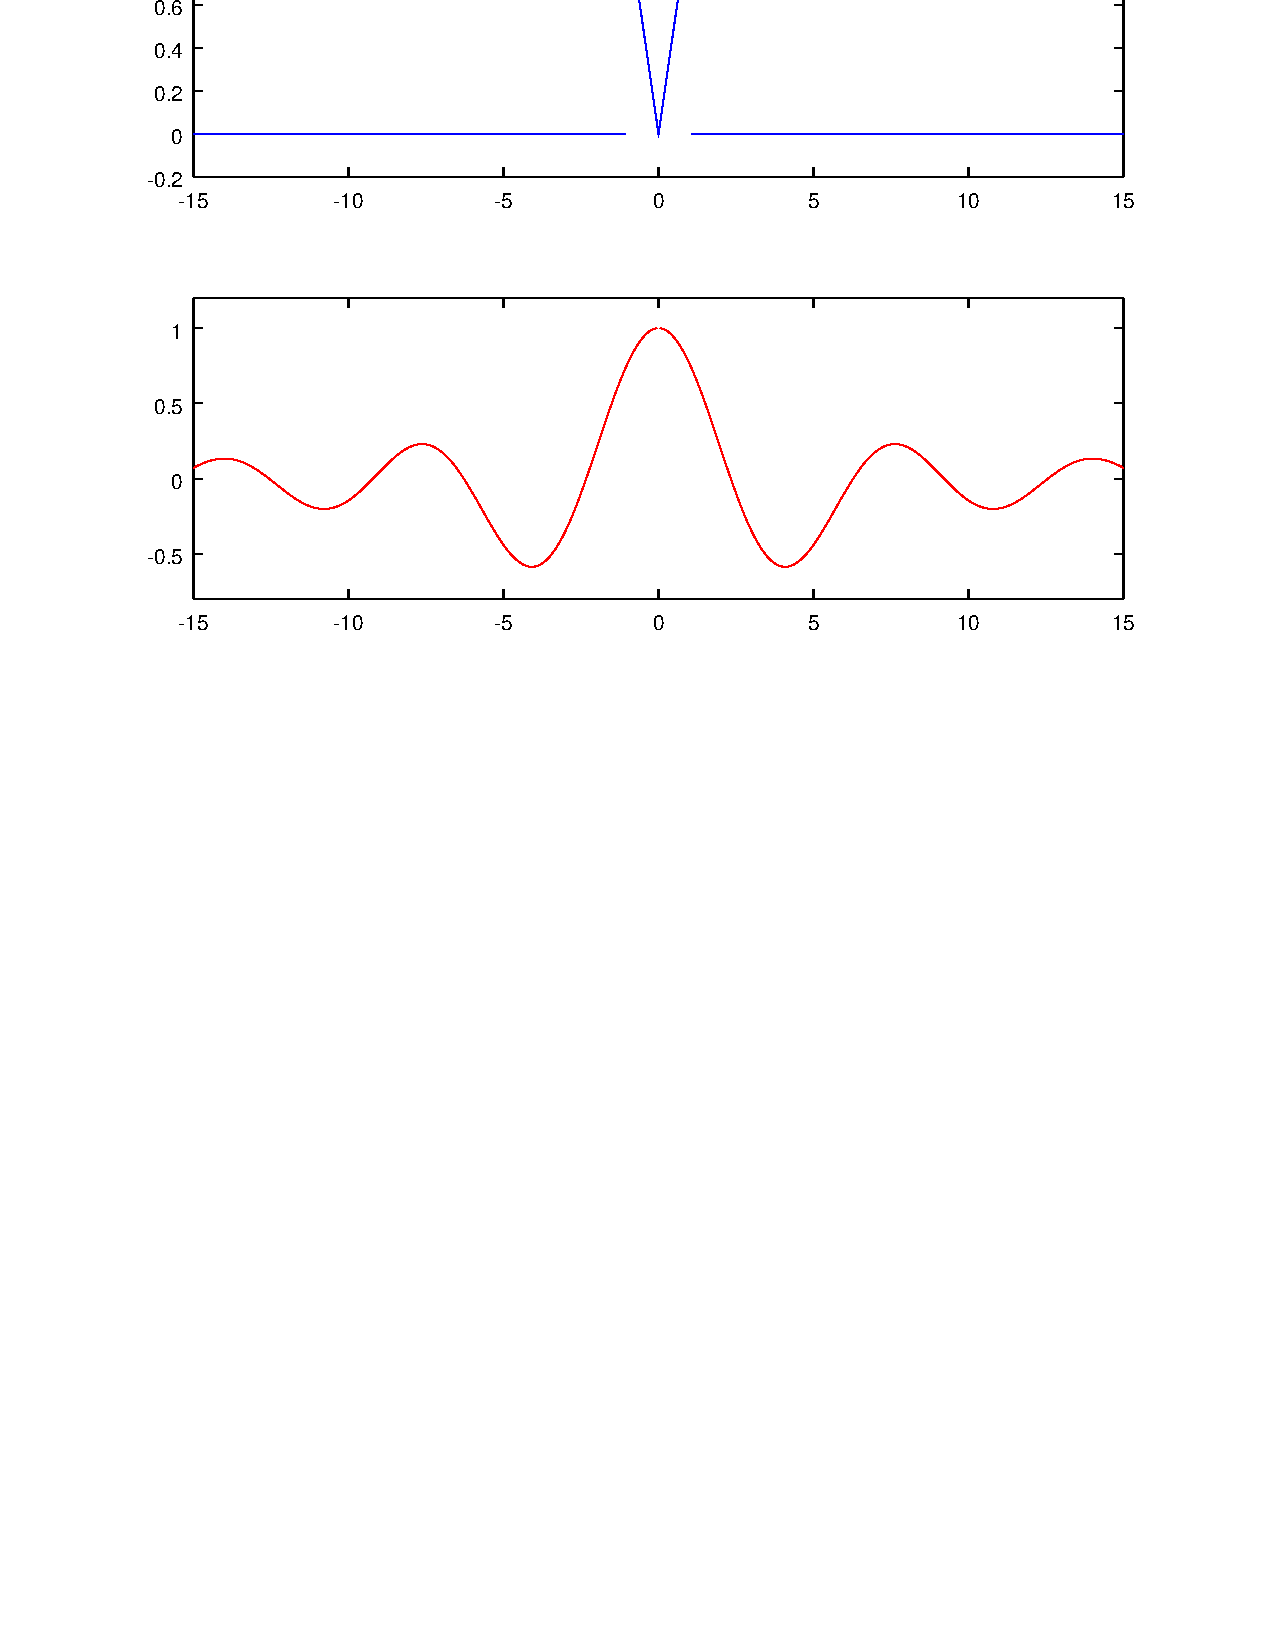
\includegraphics[scale=0.9]{abszol}
\end{center}


\feladat Számoljuk ki a következő \fv{}$FT$-ját:
\begin{equation*}
f(t) =
   \begin{cases*}
      t & $-1 \le t \le 1$ \\
      0        & egyébként
   \end{cases*}
\end{equation*}
\sect{Megoldás}
\begin{gather*}
\mhint{-\infty}{\infty}{f(t) e^{-i\omega t}}{t} \opover{1.}{=}
\mhint{-1}{1}{ t e^{-i\omega t}}{t} \opover{2.}{=}
-i\mhint{-1}{1}{t \sin(\omega t)}{t} \opover{3.}{=}\us
\opover{3.}{=}
-2i\mhint{0}{1}{t \sin(\omega t)}{t} \opover{4.}{=}
-2i\left( \mhpfv{0}{1}{t \frac{-\cos(\omega t)}{\omega}}-
\mhint{0}{1}{\frac{-\cos(\omega t)}{\omega}}{t} \right)
\opover{4.}{=}\us
-2i\left( \frac{-\cos(\omega)}{\omega}+\frac{\sin(\omega)}{\omega^2} \right)
\end{gather*}
\magy
\begin{enumerate}
\item definíciók
\item $\cos$ páros, $t\cos(\omega t)$ \kh páratlan
\item $t\sin(\omega t)$ páros
\item integrálás
\end{enumerate}


\feladat Ábrázoljuk az előző feladatbeli $FT$-at!



\feladat Számoljuk ki a következő \fv{}$FT$-ját!
\begin{equation*}
   f(t)=e^{-\gamma \vert t \vert} \kh\kh 0<\gamma \in \mathbb{R}
\end{equation*}
\sect{Megoldás}
\begin{gather*}
\mhint{-\infty}{\infty}{f(t) e^{-i\omega t}}{t} \opover{1.}{=}
2\mhint{0}{\infty}{e^{-\gamma t}\cos(\omega t)}{t} = 2A\us
A \opover{2.}{=} \frac{\gamma}{\omega} \mhint{0}{\infty}{e^{-\gamma t}\sin(\omega t)}{t} =
\frac{\gamma}{\omega} B \us
A \opover{2.}{=} \frac{1}{\gamma} - \frac{\omega}{\gamma}B \us
\opover{3.}{\implies} B = \frac{\omega}{\gamma^2+\omega^2} \opover{3}{\implies} 2A = \frac{2\gamma}{\gamma^2+\omega^2}
\end{gather*}
\magy
\begin{enumerate}
\item definíciók, $f(t)\sin(\omega t)$ páratlan, $\cos(\omega t)$ páros
\item parciális integrálások
\item egyenletrendszer megoldása, visszahelyettesítés
\end{enumerate}

\feladat Ábrázoljuk az előző feladatbeli \fv{t} és $FT$-ját különböző
$\gamma$-kra!
\sect{\href{expabszol.m}{Megoldás}}
%\lstinputlisting[style=Matlab-editor]{expabszol.m}
\begin{center}
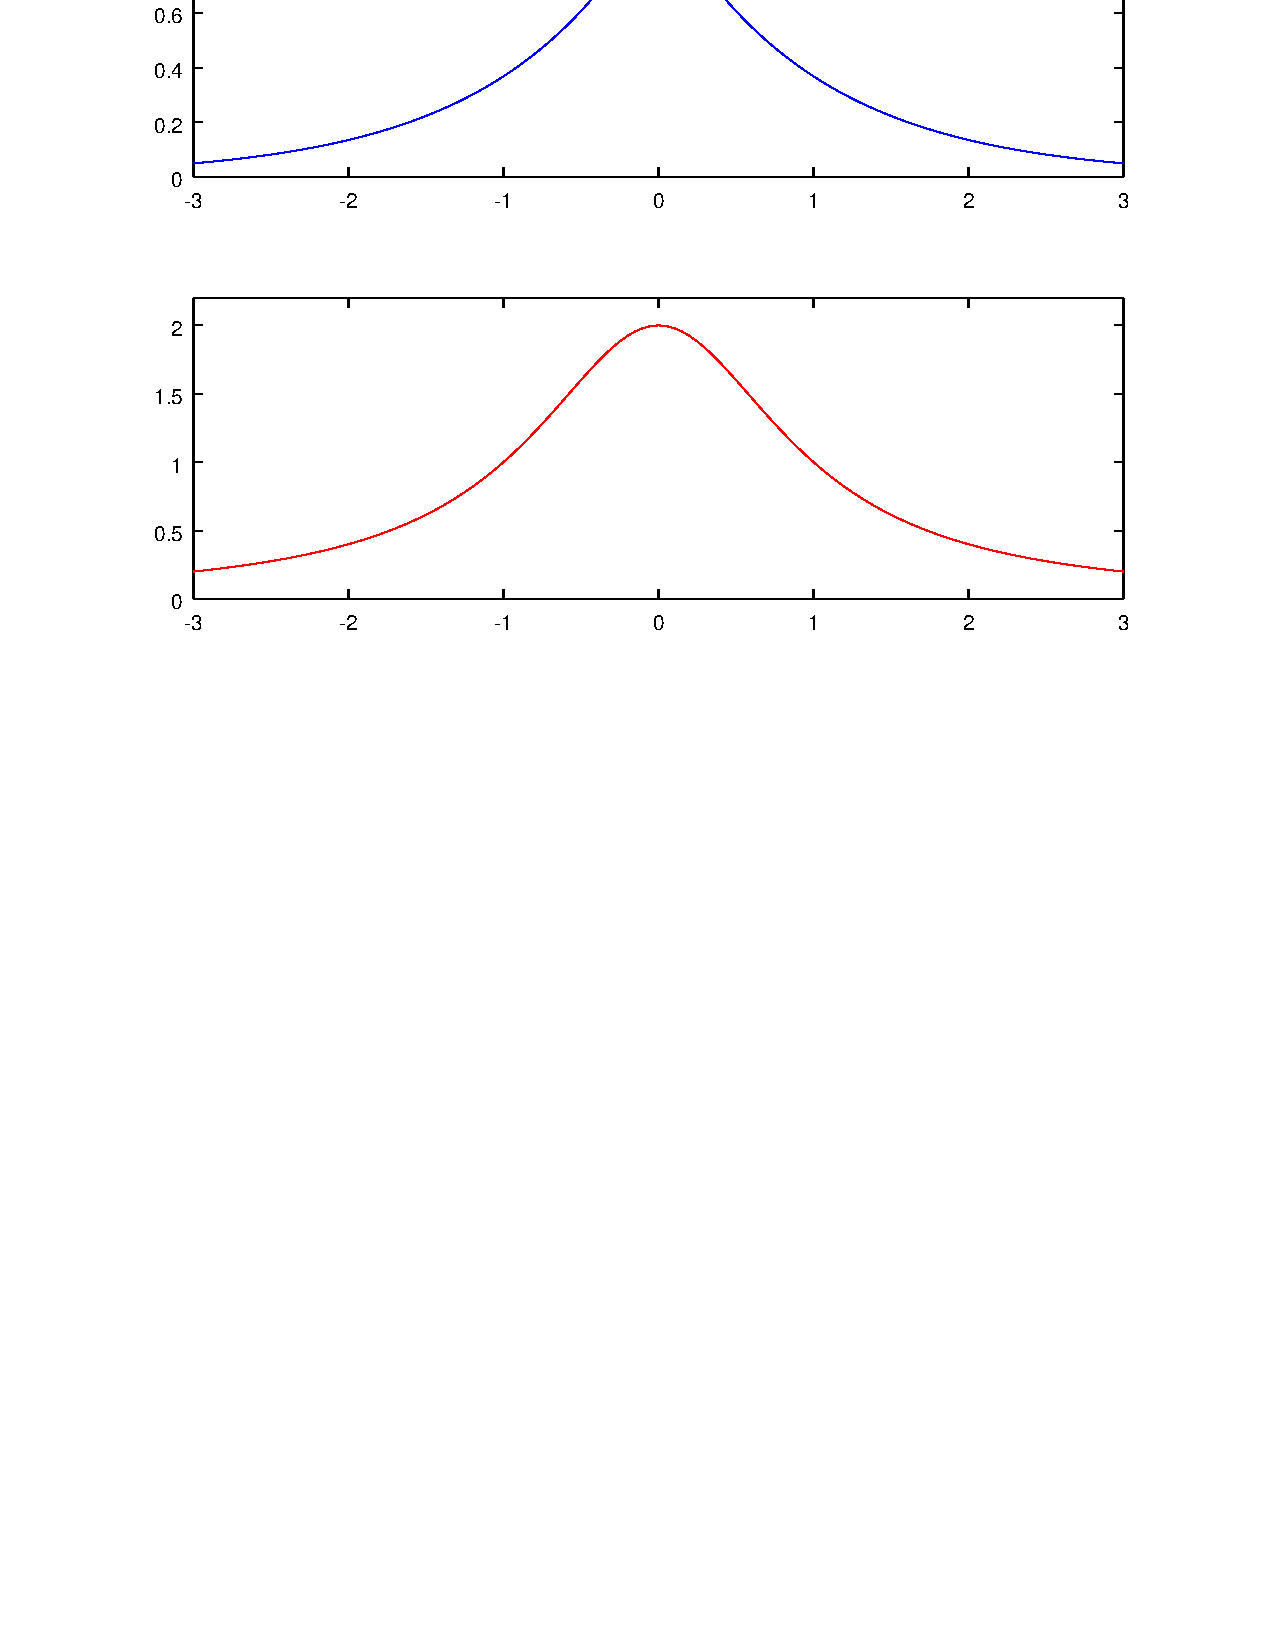
\includegraphics[scale=0.9]{expabszol}
\end{center}


\feladat Számoljuk ki a következő \fv{}$FT$-ját!
\begin{equation*}
   f(t)=e^{-\gamma t} \kh\kh 0<\gamma \in \mathbb{R}
\end{equation*}
\sect{Megoldás}
\begin{gather*}
\mhint{-\infty}{\infty}{f(t) e^{-i\omega t}}{t} \opover{1.}{=}
\mhint{0}{\infty}{e^{-\gamma t}e^{-i\omega t}}{t} =
\mhint{0}{\infty}{e^{-t(i\omega + \gamma)}}{t} = \us
\mhpfv{0}{\infty}{ -\frac{ e^{ -t(i\omega + \gamma)}}{i\omega + \gamma} }=
\frac{1}{i\omega + \gamma}
\end{gather*}



\newpage
\sect{Emlékeztető}
Az $FT$ alaptulajdonságai ($F=\mathcal{F}(f)$):
\begin{enumerate}
\item $\mathcal{F}$ lineáris
\item $(\tau_{h}f)(t)=f(t+h)$: \kh $\mathcal{F}((\tau_{h}f))(\omega) = e^{i\omega h}F(\omega)$
\kh \hfill{}(eltolás)
\item $(\delta_{a}f)(t)=f(at)$: \kh $\mathcal{F}((\delta_{a}f))(\omega) =
\frac{1}{\vert a\vert}F(\frac{\omega}{a})$ \kh \hfill{}(dilatáció)
\item $g_{n}(t)=t^{n}f(t)$ \kh $\mathcal{F}(g_n)(\omega)=i^n F^{(n)}(\omega)$
\item $\mathcal{F}(f^{(n)})(\omega)=(i\omega)^n F(\omega)$
\item $g(t)=e^{i\Omega t}f(t)$, \kh $\mathcal{F}(g)(\omega)=F(\omega-\Omega)$\hfill{}(moduláció)
\end{enumerate}

\feladat $\mathcal{F}(f)=F$ segítségével fejezzük ki az alábbi \fv{ek} $FT$-ját!
\begin{enumerate}
\item $g(t)=f(2t-3)$
\item $g(t)=\left( t^2 f(3t)\right)''$
\end{enumerate}
\sect{Megoldás}
\begin{enumerate}
\item a $2,3$ tulajdonságot használva: $\mathcal{F}(g)(\omega)=\frac{e^{-3i\omega}}{2}F(\frac{\omega}{2})$
\item a $3,4,5$ tulajdonságot használva: $\mathcal{F}(g)(\omega)= \omega^2\left( \frac{F(\frac{\omega}{3})}{3} \right)''=\frac{\omega^2 F''(\frac{\omega}{3})}{27}$
\end{enumerate}

\feladat Számítsuk ki Matlab segítségével az 
$f(x)=e^{-\vert x\vert}$
Fourier transzformáltját,
majd ábrázoljuk a függvényt és a transzformáltat egy ábrán!
\sect{\href{mlfourier.m}{Megoldás}}
\lstinputlisting[style=Matlab-editor]{mlfourier.m}



\end{document}

